% !TeX document-id = {792e8fae-71f4-5f1d-c2e4-f997d3f3f5e4}
% !TeX encoding = UTF-8
% !TeX spellcheck = en_US
% !TeX root = quest-for-greebling-v2.tex
% !TeX TXS-program:compile = txs:///pdflatex/

\documentclass[aspectratio=169]{beamer}
\usetheme{Madrid}

\usepackage{graphicx}
\usepackage{amsmath}
\usepackage{qrcode}
\usepackage{hyperref}
\usepackage{booktabs}
\usepackage{tikz}
\usetikzlibrary{arrows.meta, positioning}
\usepackage{listings}
\usepackage{xcolor}
\usepackage{helvet}
\renewcommand{\familydefault}{\sfdefault}

% --- Document Metadata ---
\title[The Quest for Greebling v2]{The Quest for Greebling}
\subtitle{Recreational AI Orchestration of Minecraft Activities}
\author[Franklin D.]{Franklin D.}
\institute[minecraft.bitsmasher.net]{Lab Research Node: \texttt{minecraft.bitsmasher.net}}
\date{\today}

% --- HIGH CONTRAST MODERN CYBERPUNK PALETTE ---
\definecolor{bgdark}{RGB}{20, 24, 33}          % Deep slate background
\definecolor{textlight}{RGB}{242, 245, 249}     % Crisp white/light-gray text
\definecolor{textmuted}{RGB}{160, 174, 192}     % Muted secondary text
\definecolor{accentcyan}{RGB}{0, 210, 255}      % Electric cyan
\definecolor{accentemerald}{RGB}{0, 230, 118}   % Emerald mirror green
\definecolor{accentamber}{RGB}{255, 179, 0}     % Alert/warning amber
\definecolor{deepslate}{RGB}{30, 37, 51}        % Card/box background
\definecolor{headerblue}{RGB}{12, 17, 26}       % Deep bar header tone
\definecolor{borderblue}{RGB}{45, 55, 72}       % Card borders
\definecolor{codebg}{RGB}{14, 18, 25}           % Code background

% --- BEAMER THEME COLOR OVERRIDES ---
\setbeamercolor{background canvas}{bg=bgdark}
\setbeamercolor{normal text}{fg=textlight}
\setbeamercolor{frametitle}{bg=headerblue, fg=accentcyan}
\setbeamercolor{frametitle right}{bg=headerblue}
\setbeamercolor{title}{bg=headerblue, fg=white}
\setbeamercolor{subtitle}{fg=accentcyan}
\setbeamercolor{item}{fg=accentcyan}
\setbeamercolor{subitem}{fg=accentemerald}
\setbeamercolor{subsubitem}{fg=accentamber}
\setbeamercolor{section in toc}{fg=white}
\setbeamercolor{section in toc shaded}{fg=textmuted}

% Footer & Header Colors
\setbeamercolor{author in head/foot}{bg=headerblue, fg=textmuted}
\setbeamercolor{title in head/foot}{bg=deepslate, fg=accentcyan}
\setbeamercolor{date in head/foot}{bg=headerblue, fg=textmuted}

% Block Colors
\setbeamercolor{block title}{bg=deepslate!90!accentcyan, fg=accentcyan}
\setbeamercolor{block body}{bg=deepslate, fg=textlight}
\setbeamercolor{block title alerted}{bg=deepslate!90!accentamber, fg=accentamber}
\setbeamercolor{block body alerted}{bg=deepslate, fg=textlight}
\setbeamercolor{block title example}{bg=deepslate!90!accentemerald, fg=accentemerald}
\setbeamercolor{block body example}{bg=deepslate, fg=textlight}

% Hide or style navigation symbols
\setbeamertemplate{navigation symbols}{}

% Presenter Note Configuration (Clean readable dark-on-light in note view)
\setbeamercolor{note page}{bg=white, fg=black}
\setbeamercolor{note title}{bg=gray!20, fg=black}
\setbeamertemplate{note page}{%
  \begin{minipage}{\textwidth}
    \color{black}
    \insertnote{}
  \end{minipage}
}

% --- CODE LISTINGS STYLE ---
\lstset{
  backgroundcolor=\color{codebg},
  basicstyle=\ttfamily\scriptsize\color{textlight},
  breaklines=true,
  captionpos=b,
  commentstyle=\color{textmuted}\itshape,
  keywordstyle=\color{accentcyan}\bfseries,
  stringstyle=\color{accentemerald},
  numbers=none,
  frame=single,
  rulecolor=\color{borderblue},
  showspaces=false,
  showstringspaces=false,
  tabsize=2
}

% --- SECTION TRANSITION SLIDES ---
\AtBeginSection[]{
  \begin{frame}[plain]
    \vfill
    \centering
    \begin{beamercolorbox}[sep=12pt,center,rounded=true,shadow=false]{frametitle}
      {\Huge \textcolor{accentcyan}{\bfseries \insertsectionhead}}\par%
      \vspace{0.4cm}
      {\small \textcolor{textmuted}{Bitsmasher Minecraft AI Research Cluster}}
    \end{beamercolorbox}
    \vfill
  \end{frame}
}


\begin{document}

% -----------------------------------------------------------------------------
% TITLE SLIDE
% -----------------------------------------------------------------------------
\begin{frame}[plain]
	\begin{columns}[c]
		\begin{column}{0.48\textwidth}
			\centering
			\includegraphics[width=0.95\textwidth]{images/Gemini_Generated_Image_e2extne2extne2ex.png}
		\end{column}
		\begin{column}{0.52\textwidth}
			\vspace{0.2cm}
			{\Huge \textcolor{accentcyan}{\bfseries The Quest for Greebling}}\par
			\vspace{0.3cm}
			{\large \textcolor{textlight}{Recreational AI Orchestration of Minecraft Activities}}\par
			\vspace{0.2cm}
			{\small \textcolor{accentemerald}{v2: Distributed Edge Inference, Emerald Mirror \& Transit Networks}}\par
			\vspace{0.6cm}
			\hrule height 1pt \relax
			\vspace{0.4cm}
			\textbf{\textcolor{white}{Franklin D.}}\par
			\footnotesize \textcolor{textmuted}{Lab Node: \texttt{minecraft.bitsmasher.net}}\par
			\footnotesize \textcolor{textmuted}{Repository: \texttt{n0ctilucent/game-skynet-minecraft}}
		\end{column}
	\end{columns}
\end{frame}

\note[itemize]{
	\item Welcome everyone to ``The Quest for Greebling v2''.
	\item Today we are exploring recreational AI orchestration of Minecraft environments using distributed hardware acceleration.
	\item This updated version covers the evolution from basic RCON scripting to our multi-node Emerald Mirror pipeline, dual-grade rail infrastructure, and edge vision interlocks.
}

% -----------------------------------------------------------------------------
% TABLE OF CONTENTS
% -----------------------------------------------------------------------------
\begin{frame}{Session Blueprint}
	\begin{columns}[t]
		\begin{column}{0.48\textwidth}
			\tableofcontents[sections={1,2,3}]
		\end{column}
		\begin{column}{0.48\textwidth}
			\tableofcontents[sections={4,5,6,7}]
		\end{column}
	\end{columns}
\end{frame}

% =============================================================================
\section{Vision \& The Art of Greebling}
% =============================================================================

\begin{frame}{What is Greebling? From Sci-Fi to Voxels}
	\begin{columns}[c]
		\begin{column}{0.55\textwidth}
			\begin{block}{Etymology \& Purpose}
				\textbf{Greebles} (or \textit{nurnies}) are intricate surface relief details added to a structure to break monotony, establish realistic scale, and create visual depth.
			\end{block}
			\begin{itemize}
				\item \textbf{Filmmaking Origins:} Coined by George Lucas and Industrial Light \& Magic (ILM) in the 1970s while kitbashing the \textit{Star Wars} Death Star and Imperial Star Destroyers.
				\item \textbf{Lego Modularity:} Widely adopted by Master Builders to infuse flat surfaces with functional texture (conduits, mechanical vents, levers).
				\item \textbf{The Minecraft Scale Dilemma:} Blocky voxels require dramatic architectural scaling to accommodate micro-relief without degenerating into visual noise.
			\end{itemize}
		\end{column}
		\begin{column}{0.45\textwidth}
			\centering
			\includegraphics[width=0.9\textwidth]{images/SKYNET_TOWER_2196.png}\par
			\vspace{0.2cm}
			\scriptsize \textcolor{textmuted}{Skynet Tower Model: Multi-layered fluted relief}
		\end{column}
	\end{columns}
\end{frame}

\note[itemize]{
	\item Greebling transforms primitive cubic geometry into convincing industrial installations.
	\item In Minecraft, placing single decorative blocks randomly looks messy; true greebling requires structured structural hierarchies (rule of three: base, pillars, girders).
}

\begin{frame}{The Minecraft Schematic Paradigm}
	\begin{columns}[c]
		\begin{column}{0.54\textwidth}
			\begin{block}{Spatial Delta vs.\ Foundation Schematics}
				Schematics capture spatial voxel topologies serialized in NBT/Sponge format for deterministic in-world deployment.
			\end{block}
			\begin{itemize}\small
				\item \textbf{Foundation Schematics:} Core skeletal anchors (structural towers, bridge pylons, load-bearing frames).
				\item \textbf{Delta Schematics:} AI-synthesized surface details with high air-block ratios wrapped over foundational geometry.
				\item \textbf{Core Objective:} Autonomous AI agents design and graft complex greebles without overwriting player spaces or dropping ticks.
			\end{itemize}
		\end{column}
		\begin{column}{0.46\textwidth}
			\centering
			\includegraphics[width=0.82\textwidth]{images/SKYNET_HOUSE_5713.png}\par
			\vspace{0.1cm}
			\scriptsize \textcolor{textmuted}{Procedural Voxel Assembly with Foundation Anchor}
		\end{column}
	\end{columns}
\end{frame}

% =============================================================================
\section{Distributed Hardware Lab \& Topology}
% =============================================================================

\begin{frame}{Physical Infrastructure: The Home Lab}
	\begin{columns}[c]
		\begin{column}{0.50\textwidth}
			\begin{itemize}
				\item \textbf{Sub-system Isolation:} Segregating high-frequency game simulation from non-deterministic neural inference.
				\item \textbf{Core Backbone:} Ubiquiti UniFi Dream Machine routing over 10G optical fiber.
				\item \textbf{10-Inch Edge Rack:} Dedicated shelf housing cluster nodes, single-board computers (SBCs), and low-voltage NPU accelerators.
				\item \textbf{Data Persistence:} \texttt{blowfish} host running OpenBSD for secure telemetry logging and digital twin storage.
			\end{itemize}
		\end{column}
		\begin{column}{0.50\textwidth}
			\centering
			\includegraphics[width=0.88\textwidth]{images/20260421_082443.jpg}\par
			\vspace{0.2cm}
			\scriptsize \textcolor{textmuted}{The 10-inch Edge Rack Lab Environment}
		\end{column}
	\end{columns}
\end{frame}

\begin{frame}{Distributed System Topology: Node Roles}
	\begin{columns}[c]
		\begin{column}{0.58\textwidth}
			\begin{itemize}\small
				\item \textbf{Chonk} (\texttt{10.10.8.60}): PaperMC 1.21.1, Java 25. Isolated 20 TPS simulation environment \& local Ollama inference.
				\item \textbf{Stargate} (\texttt{10.10.16.66}): Pi 5 (8GB). FastMCP hub, neural routing, and async telemetry receiver on port 5005.
				\item \textbf{Skynet} (\texttt{10.10.16.10}): Pi 5 (16GB) w/ Hailo-8 (26 TOPS). Real-time spatial density \& boundary safety audits.
				\item \textbf{Edge-T} (\texttt{10.10.16.4}): Asus Tinker Edge T w/ Google Coral TPU\@. Vision safety daemon \& collision check (port 8808).
				\item \textbf{Jetson Cluster} (\texttt{10.10.12.90--93}): Containerized CUDA nodes for heavy 3D voxel refinement \& delta slicing.
			\end{itemize}
		\end{column}
		\begin{column}{0.42\textwidth}
			\centering
			\includegraphics[width=0.92\textwidth]{images/greeblenet.png}\par
			\vspace{0.1cm}
			\scriptsize \textcolor{textmuted}{Distributed GreebleNet Network Routing}
		\end{column}
	\end{columns}
\end{frame}

\begin{frame}{Edge Hardware Acceleration: Hailo-8 \& Coral TPU}
	\begin{columns}[c]
		\begin{column}{0.50\textwidth}
			\centering
			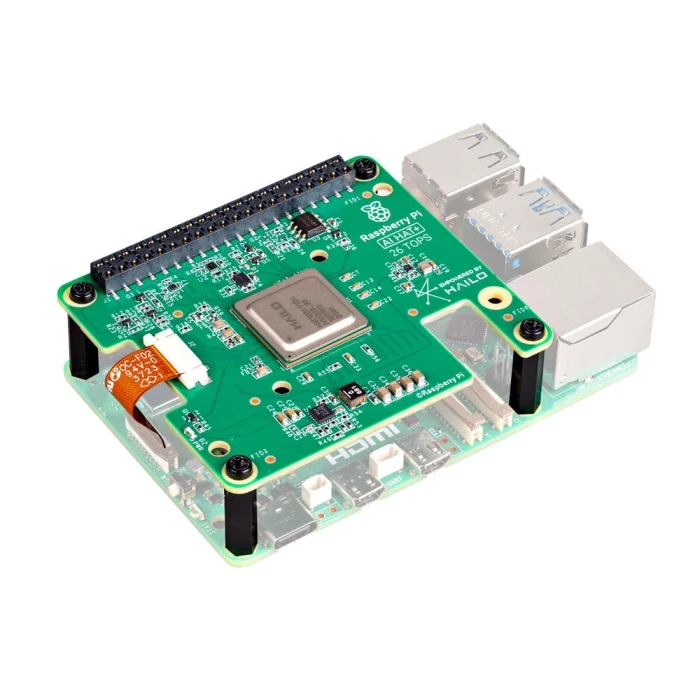
\includegraphics[width=0.48\textwidth]{images/AIHAT-26tops.png}\par
			\vspace{0.2cm}
			\begin{block}{Skynet: Hailo-8 M.2 (26 TOPS)}
				\begin{itemize}\footnotesize
					\item Executes compiled \texttt{.hef} models for 3D spatial occupancy.
					\item Prevents main-thread tick spikes during dense mesh checks.
					\item Validates schematic boundaries in under 12\,ms.
				\end{itemize}
			\end{block}
		\end{column}
		\begin{column}{0.50\textwidth}
			\centering
			\includegraphics[width=0.48\textwidth]{images/asus-tinker-edge-t.png}\par
			\vspace{0.2cm}
			\begin{block}{Edge-T: Google Coral TPU (4 TOPS)} % chktex 13
				\begin{itemize}\footnotesize
					\item Runs quantized INT8 visual inference via MDT\@.
					\item Inspects track intersections and transit switches.
					\item Enforces real-time entity safety interlocks.
				\end{itemize}
			\end{block}
		\end{column}
	\end{columns}
\end{frame}

% =============================================================================
\section{In-World Telemetry \& Electronics}
% =============================================================================

\begin{frame}[fragile]{World-Space Physical Detection \& Bridging}
	\begin{columns}[c]
		\begin{column}{0.52\textwidth}
			\begin{block}{Physical-to-Digital Transduction}
				Converting raw in-game entity mechanics into serialized distributed network events without lag.
			\end{block}
			\begin{itemize}
				\item \textbf{Detector Rails:} Placed along primary transit trunks to capture spatial cart movement.
				\item \textbf{Pulse Conditioning:} In-line 1-tick redstone repeaters condition transit pulses, preventing signal dropouts at top speed ($8\,\text{m/s}$).
				\item \textbf{Command Blocks:} Triggered directly to emit formatted JSON strings to RCON, completely bypassing JVM log verbosity.
			\end{itemize}
		\end{column}
		\begin{column}{0.48\textwidth}
			\begin{exampleblock}{Telemetry Payload Format}
\begin{lstlisting}
# Command Block Payload
tellraw @a {"text":
  "[TELEMETRY] NODE:CHONK EVENT:CART_PASS ID:TRK_04"}
\end{lstlisting}
			\end{exampleblock}
			\begin{block}{Async Daemon Ingestion}
				\texttt{chonk\_telemetry\_bridge.py} tails server buffers, extracts metadata, and dispatches JSON to Stargate port 5005 via non-blocking TCP sockets.
			\end{block}
		\end{column}
	\end{columns}
\end{frame}

\begin{frame}{Zero-Tick Observer Signal Wall Architecture}
	\begin{columns}[c]
		\begin{column}{0.50\textwidth}
			\begin{block}{The Latency Challenge}
				Standard redstone dust incurs computational ticks ($0.05\,\text{s}$ per tick), creating phase drift across long-distance railway signal corridors.
			\end{block}
			\begin{itemize}
				\item \textbf{Vertical Observer Chains:} Instantaneous 0-tick block-update propagation along vertical towers.
				\item \textbf{Physical Dispatch:} Skynet dispatches \texttt{setblock redstone\_block} (\texttt{STOP}) or \texttt{air} (\texttt{CLEAR}) directly at signal towers.
				\item \textbf{Visual Feedback:} Drivers and cart passengers observe live physical signal lamps synced with external neural routing.
			\end{itemize}
		\end{column}
		\begin{column}{0.50\textwidth}
			\centering
			\includegraphics[width=0.88\textwidth]{images/SKYNET_CASTLE_6945.png}\par
			\vspace{0.2cm}
			\scriptsize \textcolor{textmuted}{High-Tower Observer Signal Backbone Integration}
		\end{column}
	\end{columns}
\end{frame}

% =============================================================================
\section{The Emerald Mirror Pipeline}
% =============================================================================

\begin{frame}{The 4-Stage World Evolution Pipeline}
	\centering
	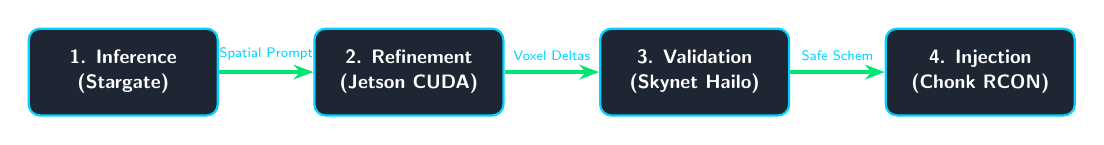
\begin{tikzpicture}[
		stage/.style={rectangle, draw=accentcyan, fill=deepslate, thick, minimum width=2.4cm, minimum height=1.1cm, align=center, rounded corners, font=\scriptsize\bfseries\color{white}},
		pflow/.style={draw=accentemerald, -{Stealth[length=2.5mm]}, ultra thick}]
		
		\node (stage1) [stage] {1. Inference\\[1pt]\scriptsize (Stargate)};
		\node (stage2) [stage, right=1.2cm of stage1] {2. Refinement\\[1pt]\scriptsize (Jetson CUDA)};
		\node (stage3) [stage, right=1.2cm of stage2] {3. Validation\\[1pt]\scriptsize (Skynet Hailo)};
		\node (stage4) [stage, right=1.2cm of stage3] {4. Injection\\[1pt]\scriptsize (Chonk RCON)};
		
		\draw [pflow] (stage1) -- node[above, font=\tiny\color{accentcyan}] {Spatial Prompt} (stage2);
		\draw [pflow] (stage2) -- node[above, font=\tiny\color{accentcyan}] {Voxel Deltas} (stage3);
		\draw [pflow] (stage3) -- node[above, font=\tiny\color{accentcyan}] {Safe Schem} (stage4);
	\end{tikzpicture}
	\vspace{0.4cm}
	
	\begin{columns}[t]
		\begin{column}{0.25\textwidth}
			\begin{block}{1. Inference}
				\tiny Ollama / FastMCP synthesizes macro concepts from world bounding snapshots.
			\end{block}
		\end{column}
		\begin{column}{0.25\textwidth}
			\begin{block}{2. Refinement}
				\tiny Jetson Edge-J executes CUDA voxel rasterization and spatial delta slicing.
			\end{block}
		\end{column}
		\begin{column}{0.25\textwidth}
			\begin{block}{3. Validation}
				\tiny Hailo-8 NPU checks containment bounds, rail clearance, and NBT integrity.
			\end{block}
		\end{column}
		\begin{column}{0.25\textwidth}
			\begin{block}{4. Injection}
				\tiny Asynchronously throttled RCON pushes block updates without dropping 20 TPS\@.
			\end{block}
		\end{column}
	\end{columns}
\end{frame}

\begin{frame}{Aesthetic Standard: The v5 Industrial Palette}
	\begin{columns}[c]
		\begin{column}{0.56\textwidth}
			\begin{block}{Transition to Industrial Brutalism}
				Engineered, high-contrast voxel specification:
			\end{block}
			\begin{itemize}\small
				\item \textbf{Vertical Columns:} Fluted $3\times 3$ \texttt{purpur\_pillar} cores with recessed stairs for deep shadowing.
				\item \textbf{Structural Girders:} \texttt{dark\_prismarine} cross-bracing.
				\item \textbf{Lighting Elements:} Inset \texttt{pearlescent\_froglight}.
				\item \textbf{Temporal Wear:} Graduated \texttt{waxed\_copper} ducting.
				\item \textbf{Foundations:} Solid \texttt{polished\_deepslate\_bricks}.
			\end{itemize}
		\end{column}
		\begin{column}{0.44\textwidth}
			\centering
			\includegraphics[width=0.88\textwidth]{images/2026-03-23_15.41.46.png}\par % chktex 8
			\vspace{0.1cm}
			\scriptsize \textcolor{textmuted}{In-World v5 Industrial Construction in AI Zone}
		\end{column}
	\end{columns}
\end{frame}

% =============================================================================
\section{Advanced Rail Transit \& Containment}
% =============================================================================

\begin{frame}{Dual-Grade Rail Architecture}
	\begin{columns}[c]
		\begin{column}{0.50\textwidth}
			\begin{block}{Ground Profile ($Y=64$)}
				\begin{itemize}\footnotesize
					\item Enclosed within AI Containment Zone Alpha.
					\item \texttt{polished\_deepslate} ballast bed at $Y=63$.
					\item Flush track bed matching factory floor grades.
					\item Strict 90-degree corner normalization.
				\end{itemize}
			\end{block}
			\vspace{0.2cm}
			\begin{block}{Elevated Arched Viaduct Profile}
				\begin{itemize}\footnotesize
					\item Spans canyons, river crossings, and exterior lines.
					\item Deepstone \& stone brick masonry arches with corbels and structural haunches.
					\item Heavy $2 \times 2$ piers with 3-block safety clearance.
					\item Iron bar parapets and cobblestone wall stanchions.
				\end{itemize}
			\end{block}
		\end{column}
		\begin{column}{0.50\textwidth}
			\centering
			\includegraphics[width=0.9\textwidth]{images/SKYNET_BRIDGE_1391.png}\par
			\vspace{0.2cm}
			\scriptsize \textcolor{textmuted}{Synthesized Elevated Arched Masonry Viaduct}
		\end{column}
	\end{columns}
\end{frame}

\begin{frame}{Station Pavilions \& Power Distribution}
	\begin{columns}[c]
		\begin{column}{0.50\textwidth}
			\centering
			\includegraphics[width=0.88\textwidth]{images/SKYNET_STATION_4478.png}\par
			\vspace{0.2cm}
			\scriptsize \textcolor{textmuted}{Autonomous $5 \times 7$ Station Terminal Pavilion}
		\end{column}
		\begin{column}{0.50\textwidth}
			\begin{block}{Covered Station Terminal Pavilions}
				\begin{itemize}\footnotesize
					\item Standardized $5 \times 7$ footprint at transit termini.
					\item Spruce boarding gates with automatic cart latching.
					\item Inset warm lantern illumination.
					\item Mandatory 3-block clearance setback from walls.
				\end{itemize}
			\end{block}
			\begin{block}{15-Block Powering Cadence}
				\begin{itemize}\footnotesize
					\item Power rails spaced exactly every 15 blocks.
					\item Hidden beneath-track redstone torches prevent roadbed clutter.
					\item Chunk-forceload batching guarantees cart transit across unpopulated server boundaries.
				\end{itemize}
			\end{block}
		\end{column}
	\end{columns}
\end{frame}

% =============================================================================
\section{Urban Greebling \& Autonomous Population}
% =============================================================================

\begin{frame}{Post-Build Urban Greebler Pipeline}
	\begin{columns}[c]
		\begin{column}{0.54\textwidth}
			\begin{block}{The Void Between Buildings}
				Early AI generation produced impressive static structures stranded on barren grass. The Urban Greebler injects systemic life.
			\end{block}
			\begin{itemize}\small
				\item \textbf{Street Infrastructure:} Iron lamp posts, redstone hydrants, and stone benches along boulevards.
				\item \textbf{Human Clutter:} Modular market stalls, crates, barrels, and tool racks along alleyways.
				\item \textbf{Rooftop Mechanicals:} Industrial HVAC chillers, ventilation ducting, and communication antennas.
			\end{itemize}
		\end{column}
		\begin{column}{0.46\textwidth}
			\centering
			\includegraphics[width=0.86\textwidth]{images/2026-03-22_21.11.13.png}\par % chktex 8
			\vspace{0.1cm}
			\scriptsize \textcolor{textmuted}{Active Urban Greebled Sector with Mechanicals}
		\end{column}
	\end{columns}
\end{frame}

\begin{frame}[fragile]{Intelligent Workstation-to-Villager Population}
	\begin{columns}[c]
		\begin{column}{0.55\textwidth}
			\begin{block}{Autonomous Demographic Assignment}
				The post-build pipeline scans interior building voxels for job sites and spawns corresponding NPC professionals.
			\end{block}
			\scriptsize
			\begin{table}
				\begin{tabular}{ll}
					\toprule
					\textbf{Detected Functional Block} & \textbf{Spawned Villager Profession} \\
					\midrule
					\texttt{minecraft:smoker} & Butcher (\texttt{minecraft:butcher}) \\
					\texttt{minecraft:blast\_furnace} & Armorer (\texttt{minecraft:armorer}) \\
					\texttt{minecraft:lectern} & Librarian (\texttt{minecraft:librarian}) \\
					\texttt{minecraft:stonecutter} & Mason (\texttt{minecraft:mason}) \\
					\texttt{minecraft:smithing\_table} & Toolsmith (\texttt{minecraft:toolsmith}) \\
					\texttt{minecraft:brewing\_stand} & Cleric (\texttt{minecraft:cleric}) \\
					\bottomrule
				\end{tabular}
			\end{table}
			\tiny Builds immediately hum with active NPC trading, pathfinding, and lived-in vitality.
		\end{column}
		\begin{column}{0.45\textwidth}
			\begin{exampleblock}{Orchestration Invocation}
\begin{lstlisting}[language=bash]
# Post-Build Orchestrator
python3 src/schematics/post_build_greebler.py \
  --schematic-dir ./schematics \
  --apply-urban \
  --populate-villagers \
  --verify-tps
\end{lstlisting}
			\end{exampleblock}
			\begin{alertblock}{TPS Watchdog Protection}
				Script halts injection immediately if live 1-minute TPS dips below $18.5$.
			\end{alertblock}
		\end{column}
	\end{columns}
\end{frame}

% =============================================================================
\section{Safety Interlocks \& Verification}
% =============================================================================

\begin{frame}[fragile]{Coral TPU Vision Interlock \& Digital Twin Registry}
	\begin{columns}[c]
		\begin{column}{0.52\textwidth}
			\begin{block}{Real-Time Coral TPU Safety Interlock}
				\begin{itemize}\footnotesize
					\item \textbf{Endpoint:} Edge-T daemon on \texttt{10.10.16.4:8808}.
					\item \textbf{Collision Prevention:} Before switches toggle, Edge-T audits an 8-block radius for players, carts, or wander mobs.
					\item \textbf{Hardware Isolation:} Inference runs purely on Coral TPU without burdening PaperMC\@.
				\end{itemize}
			\end{block}
			\begin{block}{Digital Twin: \texttt{rail\_registry.json}}
				\begin{itemize}\footnotesize
					\item Maintains authoritative dynamic state of all switches.
					\item Detects disk modifications to prevent split-brain routing.
				\end{itemize}
			\end{block}
		\end{column}
		\begin{column}{0.48\textwidth}
			\begin{exampleblock}{Digital Twin Registry Schema}
\begin{lstlisting}
{
  "switches": {
    "washington_terminus_main": {
      "coords": {"x": -1212, "y": 76, "z": -670},
      "state": true,
      "interlock_verified": true
    }
  }
}
\end{lstlisting}
			\end{exampleblock}
			\begin{block}{Automated Pytest Assurance}
				Full test coverage for containment geometry, coordinate bounds, and switch state transitions.
			\end{block}
		\end{column}
	\end{columns}
\end{frame}

\begin{frame}{Roadmap: Autonomous Multi-Agent Swarms}
	\begin{columns}[c]
		\begin{column}{0.52\textwidth}
			\begin{itemize}\small
				\item \textbf{Camera-Based Live Feedback:} Feeding BlueMap isometric streams to Hailo-8 visual inference for cosmetic grading.
				\item \textbf{Multi-Agent Builder Swarms:} Segmenting structural builds across distributed Jetson workers in parallel.
				\item \textbf{Bi-Directional Redstone Computing:} In-game ALU states modulating physical server fans and rack telemetry LEDs.
				\item \textbf{Community Federation:} Secure inter-server rail gateways linking allied Minecraft worlds.
			\end{itemize}
		\end{column}
		\begin{column}{0.48\textwidth}
			\centering
			\includegraphics[width=0.82\textwidth]{images/Gemini_Generated_Image_xz297bxz297bxz29.png}\par
			\vspace{0.1cm}
			\scriptsize \textcolor{textmuted}{Autonomous Agent Synthesis in Action}
		\end{column}
	\end{columns}
\end{frame}

\begin{frame}{Project Resources \& Discussion}
	\begin{columns}[c]
		\begin{column}{0.55\textwidth}
			{\LARGE \textcolor{accentcyan}{\bfseries Questions \& Discussion}}\par
			\vspace{0.4cm}
			\begin{itemize}\small
				\item \textbf{Repository:} \texttt{n0ctilucent/game-skynet-minecraft}
				\item \textbf{Slides PDF:} \texttt{docs/slides/quest-for-greebling-v2.pdf}
				\item \textbf{Simulation Node:} \texttt{chonk.lab.bitsmasher.net}
				\item \textbf{Author Contact:} \texttt{franklin.d@protonmail.ch}
			\end{itemize}
			\vspace{0.3cm}
			\begin{exampleblock}{Open Source Lab Stack}
				\footnotesize PaperMC $\cdot$ Hailo-8 $\cdot$ Google Coral $\cdot$ FastMCP $\cdot$ Ollama
			\end{exampleblock}
		\end{column}
		\begin{column}{0.45\textwidth}
			\centering
			\qrcode[height=2.8cm]{https://github.com/n0ctilucent/game-skynet-minecraft/raw/main/docs/slides/quest-for-greebling-v2.pdf}\par
			\vspace{0.2cm}
			\scriptsize \textcolor{textlight}{\texttt{Scan to access presentation slides}}
		\end{column}
	\end{columns}
\end{frame}

\end{document}
